This chapter provides the foundational knowledge required for the reader to comprehend the subsequent chapters of this thesis. First, the general scenario of cloud computing is presented in Section~\ref{sec:cloud}. Section \ref{sec:measuring_environmental_impact} presents how one can measure the environmental impact of cloud computing platforms. Then, an introduction to scheduling in the context of clouds is shown in Section~\ref{sec:scheduling_cloud}.  The existing approaches explored in this thesis to reduce the environmental impact of cloud computing platforms are discussed in Section~\ref{sec:carbon_responsive}, and the works used in this thesis as inspiration and baselines are presented as well. Finally,  Section~\ref{sec:summary_background} summarizes this chapter.
\section{Cloud computing}

\label{sec:cloud}

Cloud computing was introduced by the industry to address the most significant problems of e-commerce found at the time. Before the advent of cloud computing and its on-demand access to computational resources, users and companies had to purchase their own computational infrastructure to deploy their services or applications. In the event of a sudden surge in requests, it was often challenging to scale the computational infrastructure in time to handle the computational load demand. Despite its revolutionary aspects in information technology, cloud computing is not classified as a new paradigm in computer science research. As a matter of fact, it is the evolution of research into different fields of computer science, such as clusters, grids, autonomous computing, and ubiquitous computing.


One of the critical elements that enable cloud computing is virtualization technology, in which the computational resources of a physical machine are converted to virtual resources that can be shared among many users and applications---also known as multi-tenancy.  The main ideas from virtualization originate from the late 1950's and beginning of the 1960's with the multiprogramming paradigm, and today, the research on virtual machines (VMs) and containers continues to investigate the compromises outlined in the literature of multiprogramming in terms of portability---allowing the virtual resource to execute on any hardware,  performance---the impact of the additional virtual layer in the application execution in comparison to the gains regarding multi-tenancy, and security---how to isolate the interaction between different applications and the applications and the computational resources~\cite{randall2020_virtualization}.


Cloud computing platforms generally support services in three distinct levels: IaaS (Infrastructure as a Service), PaaS (Platform as a Service), and SaaS (Software as a Service)~\citep{fos08}. In the first level, Infrastructure as a Service (IaaS), the platform grants users access to hardware resources (such as processing and storage) and charges them for their usage. Services such as Amazon EC2 (Elastic Cloud Computing) Service and Amazon S3 (Simple Storage Service) are examples of IaaS clouds.   At the second level, Platform as a Service (PaaS), the provider supports a complete development, testing, and deployment environment for the application developer, which usually means that the developer will have to follow a specific fixed development model and accept restrictions on how to model the software in exchange for the scalability provided. An example is the Google App Engine. Finally, at the third level, Software as a Service (SaaS), specific applications are offered to users via the Internet, and the rate is proportional to the use of the application. We can cite the  Google Docs office applications as examples.


Modern cloud computing platforms are composed of multiple data centers geographically distributed over the world---also denominated cloud federations or multi-clouds. Figure~\ref{fig:dc_locations} illustrates the locations of the cloud data centers from Microsoft's Azure that, in total, consist of millions of physical servers~\cite{roach2021_microsoftazure}. The need for such geographically distributed infrastructure comes from meeting the demand of the huge number of users and reducing the response time for their applications, as well as for security and redundancy reasons. For example, if a data center in a region goes down because of a power problem or hacking attack, another region could temporarily receive the computational load. Finally, this distributed infrastructure enables exploring different approaches to reduce the environmental impact of operating the data centers, and more details of these strategies are given in Section~\ref{sec:carbon_responsive}.


\begin{figure}[h]
\centering
  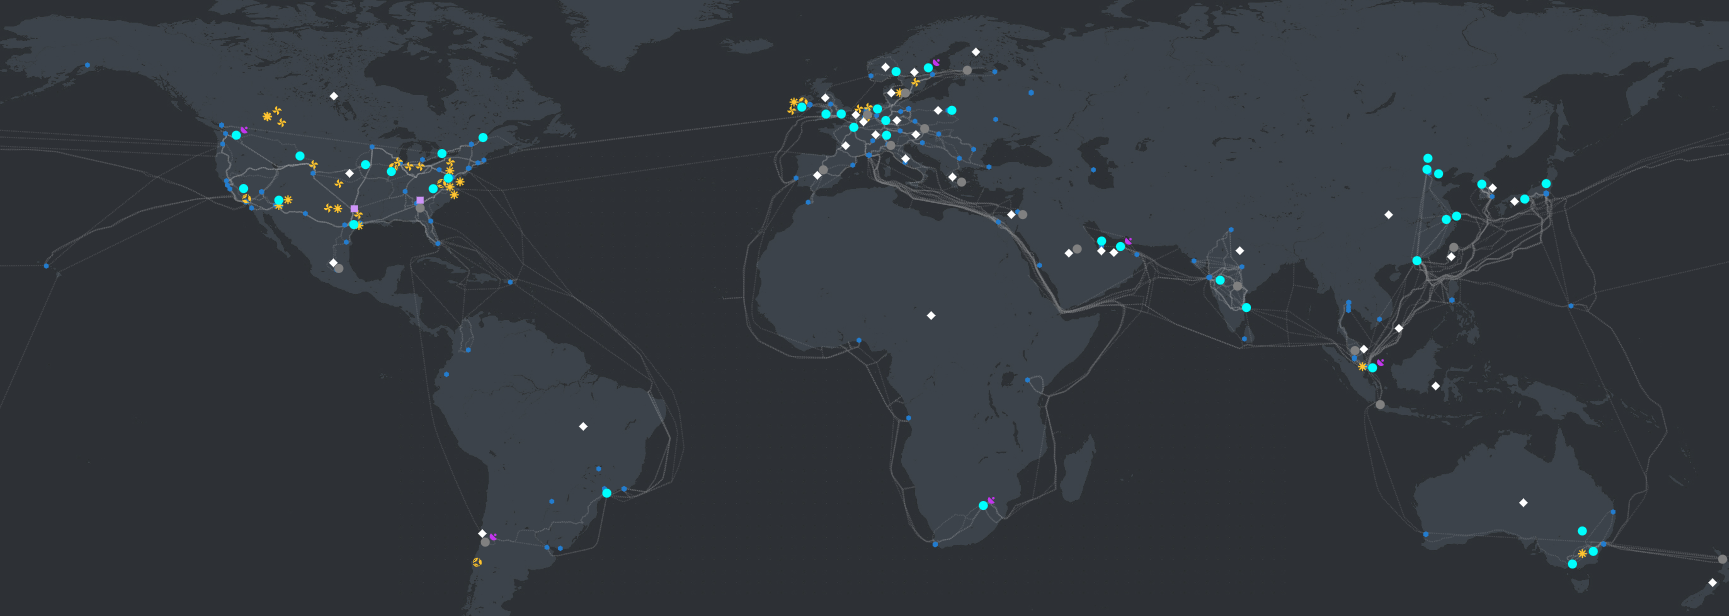
\includegraphics[width=\linewidth]{images/azure_cloud_infra.png}
  \caption{Geographic locations of Microsoft's Azure DCs. Extracted from~\cite{azure_dcs_location}.}
  \label{fig:dc_locations}
\end{figure}

\section{Measuring the environmental impact of cloud computing platforms}

\label{sec:measuring_environmental_impact}


The GHG protocol~\cite{ghgprotocol2004} was developed as a way to standardize the measurement and reporting of companies' environmental impact. It considers six types of Green Houses Gases (GHGs) of the Kyoto protocol: carbon dioxide (\ch{CO2}), methane (\ch{CH4}), sulfur hexafluoride (\ch{SF6}), nitrous oxide (\ch{N2O}), hydrofluorocarbons (HFCs), and perfluorocarbons (PFCs).


The protocol has three scopes to quantify the direct and indirect emissions:

\begin{itemize}
\item \textbf{Scope 1 - Direct GHG emissions}: Takes into account the emissions generated by sources that the company owns or has control over. In the context of cloud computing, it could come from the electricity generated when there is a power surge, and generators should be used as a backup; the transportation of products, materials, and employees using the company vehicles; and the cooling of the data center infrastructure~\cite{gupta2021_chasingcarbon}.
\item \textbf{Scope 2 - Electricity indirect GHG emissions}: Takes into account the emissions generated from the electricity consumed.
\item \textbf{Scope 3 - Other indirect GHG emissions}: This one is optional, and takes into account emissions from the production or extraction of materials and fuels bought, for example, IT equipment (such as servers and routers) as well as constructing the data center facilities. Emissions from transportation are also included in this scope if they come from vehicles not owned by the company.
\end{itemize}  

Major cloud players already provide sustainability reports and use the GHG Protocol. In the 2023 sustainability report from Meta~\cite{meta_sustainability_report_2023}, it is estimated that 1\% of the emissions came from Scope 1, less than 1\% from Scope 2, and 99\% from Scope 3. Additionally, it is stated that the operational emissions have been reduced by 94\% in comparison to 2017 thanks to the renewable energy commitments. Another remarkable example is the Google environmental report from 2023~\cite{google_sustainability_report_2023}, where it is estimated that 1\% of the emissions come from Scope 1, 24\% from Scope 2, and 74\% from Scope 3. Google also reports that most of the Scope 3 emissions come from manufacturing the hardware and capital goods they bought and constructing the data center facilities.

In this thesis, the environmental impact is only evaluated in terms of the carbon footprint---using the \ch{CO2} equivalent metric (\ch{CO2}-eq). This decision was taken due to the lack of data for measuring other environmental impacts, such as water usage, and impacts caused by extracting raw minerals to fabricate the integrated circuits.

\section{Scheduling for cloud computing platforms}
\label{sec:scheduling_cloud}

Scheduling problems are combinatorial optimization problems where, given the description of the characteristics of a computational resource set ($\alpha$) and a task set ($\beta$), the objective is to find an allocation (in time) of resources to tasks that minimize some optimization criteria ($\gamma$). These problems are denoted, generally, using the \mbox{$\alpha$ $\vert$ $\beta$ $\vert$ $\gamma$} notation, introduced by Graham~\citep{graham}. 

The most common criterion studied in problems of high-performance computing is called makespan (also denoted by $C_{\max}$), which indicates the time when the last task that makes up an application finishes its execution. When the available computational resources are identical and known previously, and we are interested in minimizing makespan---typically the case in scheduling problems in cluster and computational grids---the problem is strongly NP-hard~\citep{Garey}. This problem is denoted by $P\,\vert\,\vert\,C_{\max}$ in Graham's notation.

For the research problem explored in this thesis, $\alpha$ represents the computational resources (memory and CPU) from the servers of the data centers as well as their information about the availability of low-carbon-intensive power sources, $\beta$ represents the VM requirements in terms of execution time,  deadline, memory and CPU, and $\gamma$ represents the reduction of carbon-intensive energy consumption.

It is known---from the work of~\citet {graham} and~\citet {Garey}---that the class of greedy algorithms known as list algorithms provides fast and efficient heuristics for scheduling tasks on parallel computers. These algorithms have a $2 -1 /m$ approximation guarantee for the worst case, but are remarkably effective in practice, especially when the ratio of the number of tasks to the number of available computational resources is large. Among the most commonly used list algorithms are the Longest Processing Time first (LPT) and Shortest Processing Time first (SPT),  for homogeneous platforms, and the Heterogeneous Earliest Finish Time (HEFT) algorithm, for heterogeneous platforms.

The VM consolidation strategy illustrates an example of a scheduling problem in cloud computing enabled by virtualization. It consists of using live migrations---migrating the VM between different machines while in execution, that is, without preemption---to reallocate the VMs in order to achieve the minimum number of physical machines used, and turning off the machines that became idle to save power. The reader can check the work from~\citet{10.1145/3470972} for a systematic literature review on such techniques.


The greedy algorithms were adopted in some of the solutions proposed in this thesis, as well as most of the related works used as baselines and inspiration. The justification for such a decision is that despite not providing the optimal solution, they can provide an acceptable solution in a reasonable amount of time, which is important considering the workload size with millions of tasks and restrictions such as deadline, response time, and others. The following section presents these strategies to the reader.




\section{Carbon-Responsive Computing}

\label{sec:carbon_responsive}

Many efforts from both academia and industry are being made to reduce the environmental impact of information technology. The term Carbon-Responsive Computing was created to describe the strategies that explore moving the computational workload both in time and spatial dimensions aiming to reduce the carbon footprint of the operation~\cite{schooler2021carbonaware}.


There are three levels of Carbon-Responsive computing. In the first, Carbon-aware computing, the system knows the carbon intensity of the electricity used by its workloads or IT equipment. In the second, Carbon-responsive computing, the information about the carbon intensity is taken into account to make decisions. The final stage, Carbon-resilient computing, studies how to manage and integrate carbon-responsive elements and what modifications are needed in IT and power supply infrastructure to reduce the carbon footprint.

In this thesis, it is presented a study of the Carbon-Aware strategy follow-the-renewables---presented in Section~\ref{sec:followtherenewables}, and the Carbon-Resilient computing strategy of sizing the renewable infrastructure---discussed in Section~\ref{sec:sizing}.

\subsection{Follow-the-renewables}

\label{sec:followtherenewables}

As we saw in Section~\ref{sec:cloud}, modern cloud computing platforms are geographically distributed across the globe, having data centers in many combinations of latitudes, longitudes, and time zones. Considering that each location has a different potential for generating renewable power, and that renewable energy is intermittent---the sun only shines during the day, and the wind does not blow all the time at speeds that are sufficient to turn the wind turbine propeller---the scheduling algorithms can use this characteristic to plan the execution of the workload in the locations that have more availability of green energy. In the literature, the term ``follow-the-renewables''~\cite{shuja2016sustainable} describes this strategy. This strategy focuses on the Scope 2 of the GHG Protocol, as it schedules the workload to the location that uses less carbon-intensive power from renewable sources.

Figure~\ref{fig:ex_follow_the_renewables} is an illustration of a cloud federation's operation that adopts the follow-the-renewable strategy. The cloud federation is composed of nine data centers geographically distributed over the world, and each DC has on-site solar panels to produce green power and can also use power from the regular local electrical grid. The circles represent the locations of the data centers, and the area of the circle represents the power consumption of the DC at that instant of time. The power consumption is directly related to the amount of computational workload being executed by the DC, therefore the circle area also represents the ratio of workload allocated to the DCs. The color represents the electricity source used to supply the DC. The gray layer in the picture represents the division between night and day periods over the globe. One can observe that a higher portion of the workload was allocated to the DCs where renewable energy is being produced: the DCs located where the sun is still shining. This figure was generated from the experiments performed in this thesis. More details can be found in Chapter~\ref{chap:ccgrid}.

\begin{figure}[h]
\centering
  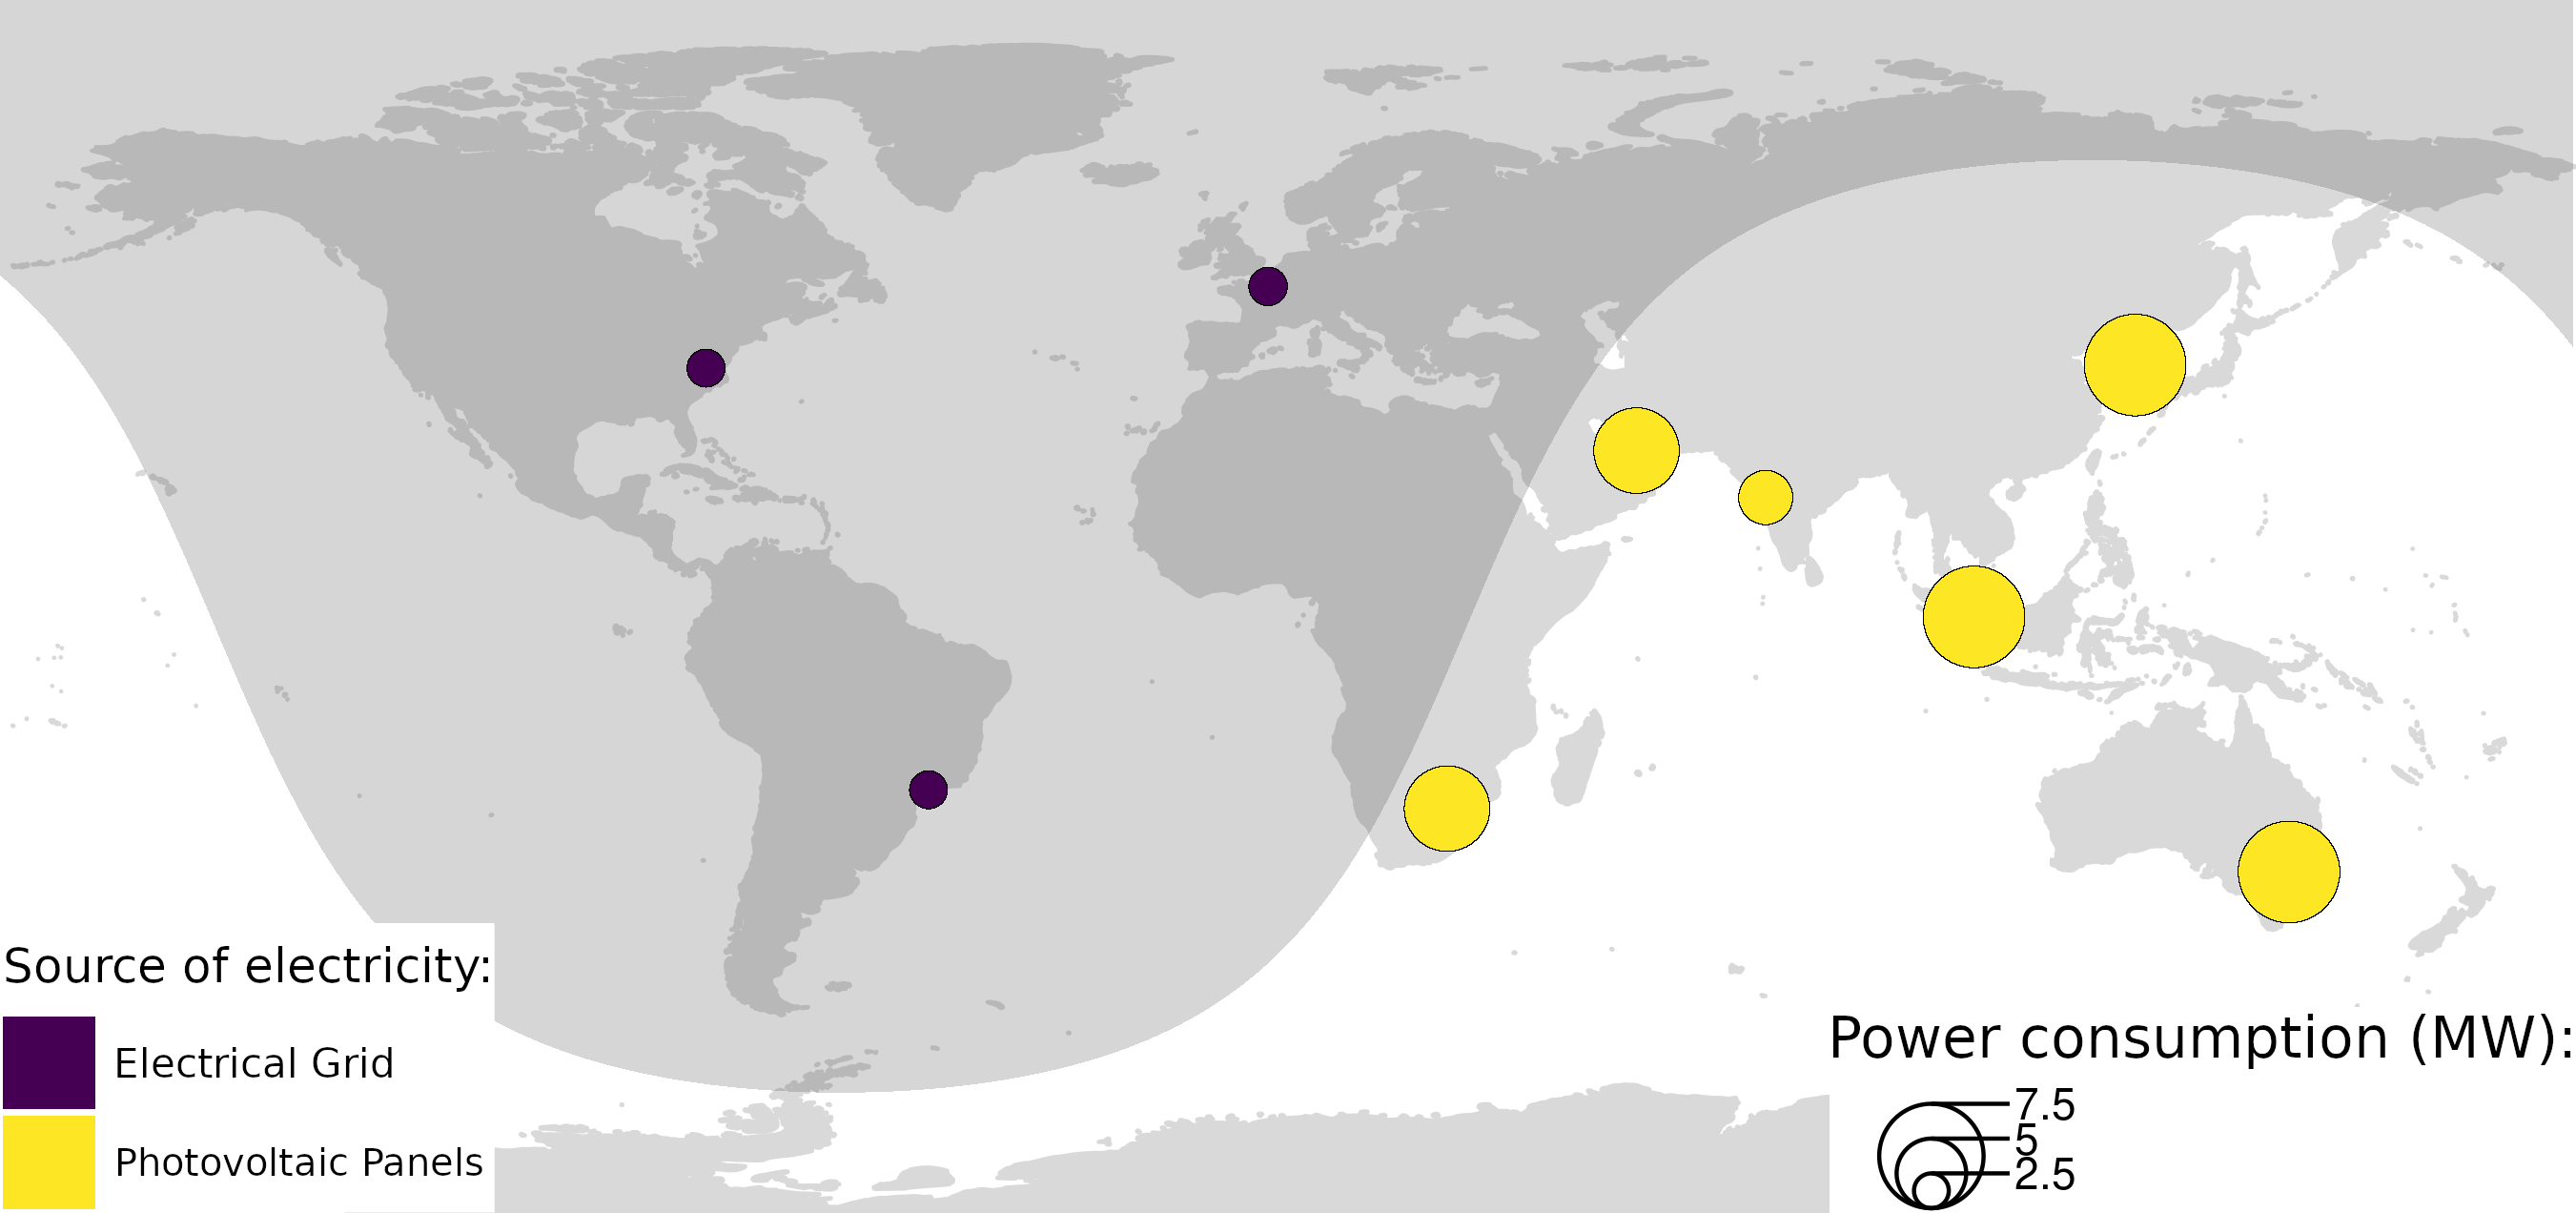
\includegraphics[width=\linewidth]{images/example_follow_the_renewables.png}
  \caption{An example of a cloud federation that adopts the follow-the-renewable strategy. Each circle represents the data center locations: its area represents the total power consumption, and the color represents the source of electricity used to supply the DC power demand. The gray layer represents the day and night periods around the world.}
  \label{fig:ex_follow_the_renewables}
\end{figure}


The work from~\citet{XU2020191} provides a comprehensive overview of the classical strategies utilized to reduce data centers' power consumption. Additionally, they present their scheduling algorithm that incorporates the ``follow-the-renewables'' to allocate the workload between the data centers located in different time zones. The optimization algorithm has the objective of minimizing the total carbon emissions of the operation while ensuring the average response time of the requests. The workload will be executed on the data centers they were allocated to, and during execution it is not possible to migrate to other DCs that may have a higher availability of green energy---no VM live migration nor VM consolidation to reduce the number of servers being used.



Reducing power consumption, the environmental impact generated by using carbon-intensive electricity, and monetary costs while not degrading workload performance were studied by~\citet{ALI2021110907}. They proposed a distributed scheduling algorithm for geographically distributed DCs with heterogeneous hardware. The algorithm has two main steps that adopt greedy heuristics. The first consists of allocating the workload to the servers given a policy (lower energy price or carbon intensity). In the second step, it is possible either to apply server consolidation to the workload in execution to reduce the number of servers in utilization (by using intra-DC migrations) or the tasks can be shifted to other data centers (inter-DC migrations) in order to use cheaper or greener electricity. The algorithm also considers that the migration's destination server might be less powerful than the server where the tasks were originally in execution, which would degrade the performance of the workload.

\citet{RUIZDUARTE2023_operation_dcs_renewables} studied the problem of operating data centers geographically distributed across the United States in terms of scheduling the workload and the power supply---that comes from the regular electrical grid, batteries, or on-site renewables. The proposed solution consisted of a Mixed Integer Linear Program (MILP) formulation that adopted follow-the-renewables for allocating and migrating the workload, and managed the decision of selecting which power source would be used. The objectives of the MILP are to minimize both costs---that originate from purchasing electricity from the grid, energy storage devices, or selling or buying carbon credits---and \ch{CO2} emissions---that originate from using carbon-intensive electricity from the regular electrical grid.

In~\citet{KHODAYARSERESHT2023_energycarbonaware_vm}, the authors study the workload scheduling problem to minimize energy consumption while avoiding violating the Service Level Agreements. The proposed solution used greedy heuristics to find the server that could run the tasks with the minimum increase in total energy consumption. If the algorithm found more than one server available, the criterion of the one that uses less carbon-intensive electricity was used to break the tie. Therefore, minimizing the emissions was the secondary objective of the algorithm, and the ``follow-the-renewables'' was only applied at this step. It is important to remind the reader that minimizing energy consumption and carbon emissions are different problems. For example, suppose DC A uses power from a grid supplied by coal power plants. In that case, it will have a carbon footprint more than 20 times higher than a DC B that consumes the same amount of power and uses photovoltaic energy--- 1001 g of\ch{CO2}-eq per kWh of electricity produced for coal power and 43  g of \ch{CO2}-eq per kWh for solar power~\cite{nrel_lifecycle_2021}. 

The studies by Camus et al.~\cite{SAGITTA,NEMESIS,SCORPIOUS} aim to optimize low-carbon-intensive energy usage in the context of data centers that have a power supply for both the regular electrical grid and locally installed solar panels. Also, these studies consider data centers that are geographically distributed, which allows for exploring ``follow-the-renewables'' strategies. The first study proposed the SAGITTA algorithm~\citep{SAGITTA}, which uses a stochastic approach to estimate renewable energy production and a greedy heuristic to allocate resources to meet the demand of virtual machines. The greedy heuristic chooses which servers in the data centers will receive the virtual machine workload considering their green energy availability and turns off those not selected to reduce the loss of renewable energy. After determining the servers to turn on or off, the algorithm tries to migrate the workload between servers in distinct data centers to use those with the most green energy availability. 

The NEMESIS algorithm~\citep{NEMESIS} is an evolution of the SAGITTA algorithm, and also uses a stochastic approach to estimate renewable energy production and greedy heuristics for VM allocation that select the servers from the data centers with the most available green energy. The main differences are that the proposed solution uses a consolidation algorithm to reduce the number of powered servers and a VM migration algorithm that considers network costs. 

The SCORPIOUS algorithm~\citep{SCORPIOUS} is an extension of the NEMESIS algorithm with a new approach: sharing excess renewable energy generated by geographically distributed data centers that have on-site solar panels installed. This approach uses SmartGrid's collective self-consumption, and the excess of green energy can be used by data centers that are not generating solar power, or when the demand is greater than the production.


Finally, ``follow-the-renewables'' approaches are feasible candidates for mitigating the intrinsic intermittent nature of renewable power, but one must not neglect its limitations. Chapter~\ref{chap:smartgreens} presents a discussion of the impact of adopting such strategies, in particular on the network and energy consumption, a proposed solution that extends the work from~\citet{NEMESIS}, and the works of~\citet{XU2020191} and~\citet{ALI2021110907} were used as baselines to evaluate the solution.


\subsection{Sizing the renewable infrastructure}


\label{sec:sizing}


There are two main options for supplying the cloud federation's power demand with low-carbon-intensive electricity. The data center owner can purchase green power from the local electricity grid that has the integration of renewables---which makes them dependent on the grid, and not all locations provide this possibility---or it can install a local renewable infrastructure in the DCs. For the latter option, the main problem is deciding the dimensions of the renewable infrastructure needed, for example, the required area of solar panels, number of wind turbines, and capacity of the batteries  (to store green power and use it when opportune) to supply the data center and minimize its carbon footprint. This problem is known as \emph{sizing}, \emph{dimensioning}, or \emph{capacity planning} in the literature. Many factors need to be considered in the sizing decision: the costs of manufacturing and operating these devices, the potential of generating power given the climate conditions and the geographic location, and the fact that these devices also present an environmental impact during their lifetime cannot be neglected as well.

The strategy sizing of the renewable infrastructure considers the Scope 1, 2, and 3 of the GHG Protocol: the direct carbon emissions from generating electricity in the DC, emissions from consuming power from the regular electrical grid, and other indirect GHG emissions that come from the manufacturing and life cycle of the renewable infrastructure and IT equipment.


Most of the scientific literature on the sizing problem for cloud data centers has focused on the scenario of a single DC. Two main approaches are investigated: i) the data center may be supplied by the regular electrical grid as a backup when the renewable power production is not sufficient, and ii) the DC is fully supplied by green energy from its on-site renewable infrastructure---which may require the adoption of energy storage devices.


The first approach---using the regular electrical grid as a backup---is adopted by the majority of works on sizing for clouds. To supply the power demand of fog DCs in a rural area in India,~\citet{padma2021_fogdcs_rural} proposed a solution that adopts a Particle Swarm Optimization strategy for sizing a smart microgrid. The optimization problem's objective is to minimize the monetary costs of buying solar panels, wind turbines, diesel generators, and batteries. Additionally, the authors propose a scheduling algorithm to maximize low-carbon-intensive energy utilization from its local renewable infrastructure. % https://doi.org/10.1007/s11276-019-02207-z

Depending on the local electricity grid and the renewable infrastructure, more renewable power can be produced than what the electrical grid can receive. In this situation, there is a curtailment, a reduction in the energy delivered when the generation exceeds the demand or there are system conditions in the grid, such as transmission congestion, minimum generation levels of thermal generators or hydropower, or back-feeding in the distribution systems~\cite{curtailment_def_2021}. 

\citet{Niaz2022_curtailment} evaluated using curtailed green energy to supply the DCs power demand and provide hydrogen to hydrogen refueling stations. The proposed solution consisted of an optimization problem that used Mixed Integer Linear Programming (MILP) with the objective of minimizing the capital costs. The modeling included natural-gas-powered combined cooling, heating, power systems, electrolyzers, hydrogen fuel cells, heat pumps, hydrogen tanks, and battery energy storage systems. The study provided three interesting results: i) the worst scenario regarding both economic and environmental aspects was to only consume power from the regular electrical grid; ii) The scenario with the minimal monetary costs was the combination of using curtailed renewable energy and power from the grid; and iii) the best solution for the environment was to consume only renewable power, however, it resulted in the highest costs.


The second main approach---using only power from the on-site renewable infrastructure without accessing the grid---is becoming more and more explored in the literature, presenting promising results. A planning methodology for a net-zero energy system---an energy system that does not emit carbon dioxide to the atmosphere~\cite{netzero_energy_system}---was discussed by~\citet{Richter2021_netzero_dcs}, which assessed the potential for a net-zero energy DC in Germany through a qualitative study. The data center is considered net-zero because its power demand would only be supplied by electricity generated by the low-carbon-intensive on-site renewable infrastructure. Power from the regular electrical grid is assumed to be highly carbon-intensive and is only used in the case of failures of the green power infrastructure. The research concluded that the DC presented a large potential to operate as a net-zero energy system, taking into account the importance of selecting proper technologies for producing electricity, increasing energy efficiency, and optimal sizing of energy storage devices. Other secondary benefits are that the marketing image and economic value can increase when the DC operates as a net-zero energy system. 

The DATAZERO~\citep{datazero} project explores the possibility of a single data center being operated exclusively from renewable energy and uses energy storage devices to try to smooth the short- and long-term intermittency. The work from~\citet{HADDAD2021100505}---part of the DATAZERO project---evaluates the possibility of using the combination of solar panels and wind turbines for supplying the DC power demand and the usage of batteries and hydrogen storage---for short- and long-term storage, respectively. The study discussed the impact of the geographic location and the computational workload that must be executed in the resulting sizing---number of servers, dimensions of the renewable power sources, and capacity of the energy storage devices.

Another work from the DATAZERO project evaluated how to reduce oversizing, that is, manufacturing more renewable infrastructure than needed, in DCs powered by green energy~\citep{manal2022}. The classical sizing approaches are very sensitive to variations in the inputs, as there are a few days when there is a peak in computational demand for the workload or low renewable production. The proposed solution evaluated how to minimize the oversizing and the impact in terms of Quality of Service and on the dimensions of the renewable infrastructure. A binary search strategy was adopted to find the best relevant sizing, in contrast to the previous studies that used MILP approaches.

Other research areas explored in the scientific literature analyze the sizing of particular elements, such as the electrical infrastructure. ~\citet{sheme2018_batsize} investigated the usage of batteries as an energy storage device and their size to supply 50\% of the DC's total energy demand using power from renewable sources. For the experiments, the authors developed a simulator that receives information on the PV area and capacity of the batteries as input, and different geographic locations were considered: Finland, Crete, and Nigeria. The results highlight the different potential of the geographic locations: Nigeria presented the smallest area of solar panels required: 17\% less than Crete and 45\% less than Finland. Additionally, Finland requires a battery with 39 times more capacity than Nigeria---even if it receives 15\% less solar energy, and Crete needs a battery with a capacity 27\% higher than Nigeria.

Most studies in the literature focus on dimensioning the renewable infrastructure for a single data center. A similar trend can be observed in the context of scheduling problems for DCs powered by green energy:  a literature review on recent publications on the subject of DCs that are supplied by renewable energy was made by~\citet{SONG2022326}, and the results show that over 100 publications, only around 25\% considered geographically distributed data centers partially powered by renewable energy. Additionally, the authors reported that most research on integrating renewable sources in cloud data centers focuses on the scheduling of the workload, and few articles analyze the dimensioning of the renewable infrastructure.

The Carbon Explorer framework~\cite{acun2022holistic} explored sizing for multiple geographically distributed DCs. The study's objective is to supply DCs located in the United States exclusively with renewable power, and three strategies were used: i) only use green power; ii) use renewable power and energy storage devices; and iii) use green energy and workload scheduling. It is assumed that the DCs have access to low-carbon intensive power from the regular electrical grid---solar, wind, or both---and additional renewable infrastructure will be built---PV panels, wind turbines, and batteries, taking into account the emissions of manufacturing. The study performed an exhaustive search to evaluate the possible scenarios. In conclusion, the authors report that, when taking into account the scenario of geographically distributed data centers and the manufacturing carbon emissions of the renewable infrastructure, there may be better solutions than powering the cloud federation exclusively with green power. Finally, deciding the optimal solution is still an open research question for future work.


This thesis explored the dimensioning of geographically distributed data centers worldwide. The proposed solution combined both ``follow-the-renewables'' for scheduling the workload and sizing the renewable infrastructure to reduce the carbon footprint of a global cloud federation. Compared to the Carbon Explorer framework, our proposed solution considers the use of the local electrical grid when feasible, given that it may have the presence of low-carbon-intensive power sources. Finally, our model uses a linear program formulation, in contrast to most of the works in the literature that use MILP.

In Chapter~\ref{chap:ccgrid}, the reader is introduced to our initial modeling of the problem and the evaluation of the short-term scenario (1 year) for reducing the carbon footprint of operating a cloud federation. In Chapter~\ref{chap:ccgrid-extension}, an extension of the modeling is presented, focusing on the long-term operation, taking into account the life-cycle of the renewable infrastructure, another source for renewable power, scheduling strategies to reduce the carbon footprint further, and manufacturing servers taking into account their carbon footprint. Additionally,  one new dimension of the problem is explored: the monetary costs of reducing the environmental impact with on-site renewable infrastructure.




\section{Summary}
\label{sec:summary_background}
This chapter presented an overview of the context of cloud computing, how it is possible to measure the environmental impact of the cloud computing platforms using the GHG protocol, scheduling, and the concept of carbon-responsive computing to describe the strategies for reducing its environmental impact, in particular the follow-the-renewables and the sizing that are explored in this thesis. The content presented in this chapter should provide the reader with adequate information to comprehend the succeeding chapters of this thesis.
